\documentclass[10pt]{article}
\usepackage[utf8]{inputenc}
\usepackage[doublespacing]{setspace}
\usepackage{textcomp}
\usepackage{amsmath,amssymb,amsthm}
\usepackage{fancyhdr}
\usepackage{lastpage}
\usepackage[]{hyperref}
\usepackage[pdftex]{graphicx}
\usepackage{ctex}
\usepackage{booktabs}
\usepackage{subfigure}
\usepackage{titlesec}
\usepackage{listings}
\usepackage{enumerate}
\usepackage{bm}
\usepackage{float}
\usepackage{url}
\usepackage[english]{babel}
\usepackage[dvipsnames]{xcolor}
\usepackage{scalerel}
\usepackage[margin=1.25in]{geometry}
%\allowdisplaybreaks
\renewcommand{\contentsname}{\centerline{Contents}}
\pagestyle{fancy}
\author{D}
\def\name{D}
\lhead{Multivariate Statistical Methods}
\chead{}
\rhead{\name}
\cfoot{-\space\thepage\space-}
\newtheorem{prob}{\bm{$Problem$}}
\newtheorem{bonus}{\bm{$Bonus\;Problem$}}
\newcommand{\tabincell}[2]{\begin{tabular}{@{}#1@{}}#2\end{tabular}}
\CTEXoptions[today=old]
\newcommand\reallywidehat[1]{\arraycolsep=0pt\relax%
\begin{array}{c}
\stretchto{
  \scaleto{
    \scalerel*[\widthof{\ensuremath{#1}}]{\kern-.5pt\bigwedge\kern-.5pt}
    {\rule[-\textheight/2]{1ex}{\textheight}} %WIDTH-LIMITED BIG WEDGE
  }{\textheight} %
}{0.5ex}\\           % THIS SQUEEZES THE WEDGE TO 0.5ex HEIGHT
#1\\                 % THIS STACKS THE WEDGE ATOP THE ARGUMENT
\rule{-1ex}{0ex}
\end{array}
}

\begin{document}

\title{Assignment Two}
\date{\today}
\maketitle
\thispagestyle{fancy}

\newpage

\begin{prob}
\end{prob}
\begin{enumerate}[1)]
\vspace{3mm}

\item
Plot with R.
\begin{figure}[H]
  \centering
  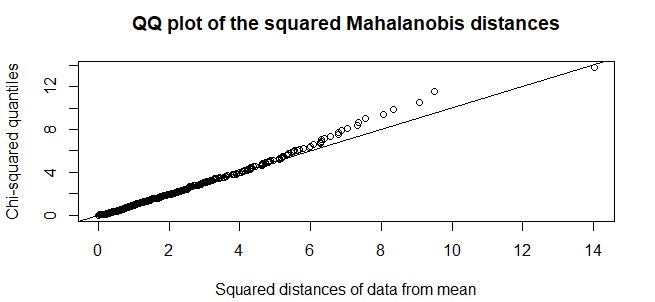
\includegraphics[scale=0.45]{p11b.png}
  %\caption{QQ plot of the squared Mahalanobis distances for {\fontfamily{ptm}\ttfamily Test} and {\fontfamily{ptm}\ttfamily Exam}}
\end{figure}
Yes, they are approximately bivariate normally distributed, despite a small amount of outliers. We observe the points generally fall on a straight line with slight skewness. The points that are close to the center should have high frequency, and those away from the center have low frequency. However, the way we treat missingness affects the result. In the case above, we select {\fontfamily{ptm}\ttfamily Test} and {\fontfamily{ptm}\ttfamily Exam}, and only remove the rows with missing values in any of them or both, with {\fontfamily{ptm}\ttfamily is.na}, keeping 494 students. If we use {\fontfamily{ptm}\ttfamily na.omit} to filter out about $\frac{1}{3}$ of the students and keep 378 students, it gives another story and the plot below displays more linearity with less skewness.
\begin{figure}[H]
  \centering
  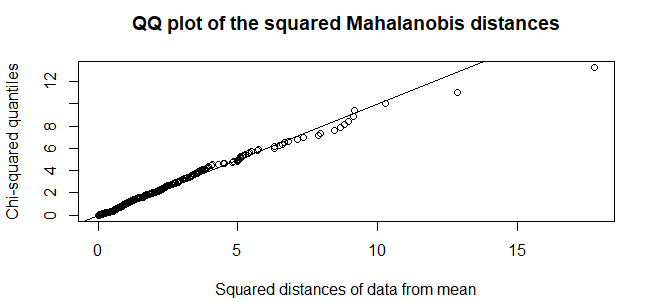
\includegraphics[scale=0.45]{p11c.png}
  %\caption{QQ plot of the squared Mahalanobis distances for {\fontfamily{ptm}\ttfamily Test} and {\fontfamily{ptm}\ttfamily Exam}}
\end{figure}

\item
We use forward selection, AIC as the information criteria and a log scale on {\fontfamily{ptm}\ttfamily Exam}.
\begin{table}[H]
\centering
\scriptsize
\begin{tabular}{l|l}
Model & AIC \\ \hline
$log(Exam)=\beta_0$ & -518.98 \\ \hline
$log(Exam)=\beta_0+\beta_1 Assignment$ & -628.31 \\
$log(Exam)=\beta_0+\beta_1 Test$ & -622.11 \\
$log(Exam)=\beta_0+\beta_1 S2$ & -595.91 \\
$log(Exam)=\beta_0+\beta_1 Project$ & -554.02 \\
$log(Exam)=\beta_0+\beta_1 S1$ & -523.56 \\ \hline
$log(Exam)=\beta_0+\beta_1 Assignment+\beta_2 Test$ & -683.57 \\
$log(Exam)=\beta_0+\beta_1 Assignment+\beta_2 S2$ & -641.77 \\
$log(Exam)=\beta_0+\beta_1 Assignment+\beta_2 Project$ & -634.53 \\
$log(Exam)=\beta_0+\beta_1 Assignment+\beta_2 S1$ & -629.09 \\ \hline
$log(Exam)=\beta_0+\beta_1 Assignment+\beta_2 Test+\beta_3 S2$ & -703.64 \\
$log(Exam)=\beta_0+\beta_1 Assignment+\beta_2 Test+\beta_3 Project$ & -685.33 \\
$log(Exam)=\beta_0+\beta_1 Assignment+\beta_2 Test+\beta_3 S1$ & -683.20 \\ \hline
$log(Exam)=\beta_0+\beta_1 Assignment+\beta_2 Test+\beta_3 S2+\beta_4 Project$ & -705.41 \\
$log(Exam)=\beta_0+\beta_1 Assignment+\beta_2 Test+\beta_3 S2+\beta_4 S1$ & -703.13 \\
\end{tabular}
%\caption{Models by forward selection}
\end{table}
Using {\fontfamily{ptm}\ttfamily na.omit} in R, we filter out the rows with at least one missing value, and using {\fontfamily{ptm}\ttfamily step}, we get the result above. We begin without any variables and get the AIC -518.98. Then we add the first variable, find adding {\fontfamily{ptm}\ttfamily Assignment} gives the smallest AIC -628.31 and we choose {\fontfamily{ptm}\ttfamily Assignment} as the first variable. Repeating the steps, we add the second variable {\fontfamily{ptm}\ttfamily Test} with the smallest AIC -683.57, the third variable {\fontfamily{ptm}\ttfamily S2} with AIC -703.64 and the last variable {\fontfamily{ptm}\ttfamily Project} with AIC -705.41. We do not include {\fontfamily{ptm}\ttfamily S1} since adding it to the model in each step always produces a greater AIC.\\
The minimal adequate model we get with the estimated coefficients is
\begin{align*}
log(Exam)=2.67+0.02Assignment+0.02Test+0.16S2+0.05Project.
\end{align*}
With {\fontfamily{ptm}\ttfamily summary}, we may conclude that {\fontfamily{ptm}\ttfamily Test}, {\fontfamily{ptm}\ttfamily Assignment} and {\fontfamily{ptm}\ttfamily S2} are good explanatory variables for the exam marks. The project probably involves group work and extra study less relevant to the exam. Students may not engage in {\fontfamily{ptm}\ttfamily S1} for having studied the contents in their high school and {\fontfamily{ptm}\ttfamily S1} has a longer timespan with the exam. So we may include {\fontfamily{ptm}\ttfamily Project} and do not include {\fontfamily{ptm}\ttfamily S1}.\\


\item
We compare the two models, using {\fontfamily{ptm}\ttfamily summary} in R. In the maximal model, the term {\fontfamily{ptm}\ttfamily S1} is very insignificant with t-statistic -1.298 and the term {\fontfamily{ptm}\ttfamily Project} is slightly insignificant with t-statistic 1.986; in the minimal adequate model, the term {\fontfamily{ptm}\ttfamily Project} is slightly insignificant with t-statistic 1.933. The F-statistic for the maximal model is 50.6; the F-statistic for the minimal adequate model is 62.72. It is reasonable to exclude {\fontfamily{ptm}\ttfamily S1} for its poor explanation. The AIC for the maximal model is -705.12; the AIC for the minimal adequate model is -705.41. The adjusted $R^2$ for the maximal model is 0.3968; The adjusted $R^2$ for the minimal adequate model is 0.3957. The p-values less than 2.2e-16 for both are almost the same. They all show little performance is lost by excluding {\fontfamily{ptm}\ttfamily S1}. Despite little performance, we still suggest excluding {\fontfamily{ptm}\ttfamily S1}.\\

\item
The following results are after using {\fontfamily{ptm}\ttfamily na.omit}, so many outliers may have been filtered out.\\
With {\fontfamily{ptm}\ttfamily plot}, we get four regression diagnostic plots. In the Residuals vs Fitted plot, a bow-shape curve is returned and it shows a slight non-linear relationship that is left out in the residuals but not explained by the model. In the Normal Q-Q plot, the points in the middle are lined well so the residuals are normally distributed, but on the two sides, especially the right, the residuals are not lined well so not normally distributed. In the Scale-Location plot, a slightly downward line appears, but generally the residuals appear randomly spread. In the Residuals vs Leverage plot, all points are inside the 0.5 Cook's distance line so no influential outliers are found.\footnote{\;Kim, B. (2015, September 21). Understanding diagnostic plots for linear regression analysis. In University of Virginia Library. Retrieved 3:57, May 4, 2020, from \url{https://data.library.virginia.edu/diagnostic-plots}.}\\
In spite of a few outliers that influence the regression slightly, generally there are not any OLS regression assumption violated. Using the Residuals vs Leverage plot, we conclude that there are not any points that can influence the linear regression with high leverage. It is reasonable since the marks are within a grading range and no large influential values are generated.

\end{enumerate}

\begin{prob}
\end{prob}
\begin{enumerate}[1)]
\vspace{3mm}

\item
We get the required matrix plot and correlation matrix with R.
\begin{figure}[H]
  \centering
  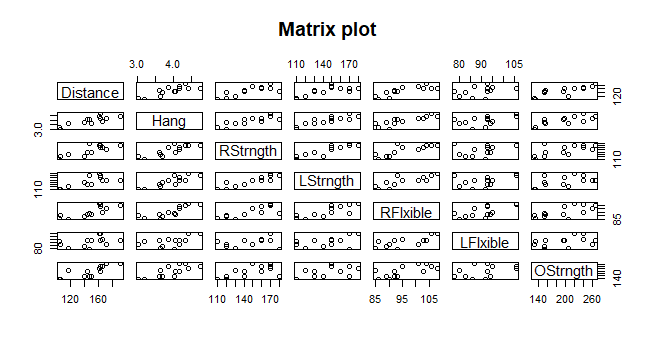
\includegraphics[scale=0.6]{p21b.png}
  %\caption{Matrix plot}
\end{figure}
\begin{table}[H]
\centering
\scriptsize
\begin{tabular}{llllllll}
\multicolumn{8}{c}{Correlation matrix}                                            \\ \hline
         & Distance & Hang & RStrngth & LStrngth & RFlxible & LFlxible & OStrngth \\
Distance & 1.00     & 0.82 & 0.79     & 0.74     & 0.81     & 0.41     & 0.80     \\
Hang     & 0.82     & 1.00 & 0.83     & 0.86     & 0.85     & 0.53     & 0.76     \\
RStrngth & 0.79     & 0.83 & 1.00     & 0.90     & 0.77     & 0.36     & 0.61     \\
LStrngth & 0.74     & 0.86 & 0.90     & 1.00     & 0.81     & 0.42     & 0.52     \\
RFlxible & 0.81     & 0.85 & 0.77     & 0.81     & 1.00     & 0.69     & 0.69     \\
LFlxible & 0.41     & 0.53 & 0.36     & 0.42     & 0.69     & 1.00     & 0.41     \\
OStrngth & 0.80     & 0.76 & 0.61     & 0.52     & 0.69     & 0.41     & 1.00
\end{tabular}
%\caption{Correlation matrix}
\end{table}
This dataset is small and without missingness. We also need to pay attention to the issue of correlation and causation. We define the correlation above 0.7 as strong, that between 0.4 and 0.7 as moderate and that below 0.4 as weak.\\
For the response variable {\fontfamily{ptm}\ttfamily Distance}, all the explanatory variables have positive correlation with it. {\fontfamily{ptm}\ttfamily RStrength}, {\fontfamily{ptm}\ttfamily LStrength}, {\fontfamily{ptm}\ttfamily RFlexibility} and {\fontfamily{ptm}\ttfamily Overall Strength} have a strong correlation, as 0.79, 0.74, 0.81 and 0.8 respectively; {\fontfamily{ptm}\ttfamily LFlexibility} has a moderate correlation, as 0.41. For the response variable {\fontfamily{ptm}\ttfamily Hang}, all the explanatory variables have positive correlation with it. {\fontfamily{ptm}\ttfamily RStrength}, {\fontfamily{ptm}\ttfamily LStrength}, {\fontfamily{ptm}\ttfamily RFlexibility} and {\fontfamily{ptm}\ttfamily Overall Strength} have a strong correlation, as 0.83, 0.86, 0.85 and 0.76 respectively; {\fontfamily{ptm}\ttfamily LFlexibility} has a moderate correlation, as 0.53.\\
Positive correlations among the explanatory variables can be observed. For example, {\fontfamily{ptm}\ttfamily RStrength} has a strong correlation with {\fontfamily{ptm}\ttfamily LStrength} and {\fontfamily{ptm}\ttfamily RFlexibility} and a moderate correlation with {\fontfamily{ptm}\ttfamily Overall Strength}. {\fontfamily{ptm}\ttfamily LStrength} has a strong correlation with {\fontfamily{ptm}\ttfamily RStrength} and {\fontfamily{ptm}\ttfamily RFlexibility}. \linebreak{\fontfamily{ptm}\ttfamily LFlexibility} and {\fontfamily{ptm}\ttfamily Overall Strength} also have moderate correlations with the other explanatory variables.\\
The result implies that a footballer usually practices both legs' strength at the same time, for the strong correlation between {\fontfamily{ptm}\ttfamily RStrength} and {\fontfamily{ptm}\ttfamily LStrength}; they are less likely do so on both hamstring muscles' flexibility, for their moderate correlation. Right legs are likely to be the dominant leg since it has strong correlations with the other variables than left legs. Good leg strength may indicate good hamstring muscle flexibility, and vice versa, but we must investigate the causation; training may increase the leg strength and the hamstring muscle flexibility together.\\

\item
With {\fontfamily{ptm}\ttfamily lm} and {\fontfamily{ptm}\ttfamily summary} in R, we build a model with {\fontfamily{ptm}\ttfamily log(Disntance)} as the response variable and get its summary. For the model, the adjusted $R^2$ is 0.66 and moderate; the F-statistic is 5.663 and low; the p-value is 0.02 and fine; overally, the model is fine. For the coefficients, besides the intercept with a significant t-statistic 7.82, the other coefficients for the explanatory variables all have a insignificant t-statistic, indicating we are unlikely to reject the null hypothesis that allows us to conclude that there is a relationship between {\fontfamily{ptm}\ttfamily Distance} and these explanatory variables, which is an evidence of multicollinearity.\\
The reason why the ANOVA and the individual estimated coefficients produce opposite evaluations for the model is that the combination of the explanatory variables can explain the response variable well, but individual variables do not. This phenomenon indicates the multicollinearity among the explanatory variables. When we use a single explanatory variable, say {\fontfamily{ptm}\ttfamily RStrength}, we can get the coefficient t-statistic is significant.\\
In addition, we use {\fontfamily{ptm}\ttfamily cov2cor} to see the correlations between two estimated coefficients and the multicollinearity. We get that $CORR[\hat{\beta}_{RStrength},\hat{\beta}_{LStrength}]$ is -0.71, $CORR[\hat{\beta}_0,\hat{\beta}_{RFlexibility}]$ is -0.68 and $CORR[\hat{\beta}_{RFlexibility},\hat{\beta}_{LFlexibility}]$ is -0.65. These imply {\fontfamily{ptm}\ttfamily Overall Strength} is likely to be selected by model selection and the flexibility variables are not.\\

\item
Compute with R.
\begin{table}[H]
\centering
\scriptsize
\begin{tabular}{l|l|l}
Selection & Model & AIC \\ \hline
Forward selection & $log(Distance)=\beta_0+\beta_1 RStrngth+\beta_2 OStrgnth$ & -58.09\\
Backward selection & $log(Distance)=\beta_0+\beta_1 LStrngth+\beta_2 OStrgnth$ & -58.67\\
Stepwise forward selection & $log(Distance)=\beta_0+\beta_1 RStrngth+\beta_2 OStrgnth$ & -58.09\\
Stepwise backward selection & $log(Distance)=\beta_0+\beta_1 LStrngth+\beta_2 OStrgnth$ & -58.67\\
\end{tabular}
%\caption{Models by different selections}
\end{table}

The results of forward, backward and stepwise selection for multiple regression of Distance are not the same. The models by forward selection and stepwise forward selection select {\fontfamily{ptm}\ttfamily RStrengt)} and {\fontfamily{ptm}\ttfamily Overall Strength} as its explanatory variables, with a slightly greater AIC -58.09; the models by backward selection and stepwise backward selection select {\fontfamily{ptm}\ttfamily LStrengt)} and {\fontfamily{ptm}\ttfamily Overall Strength} as its explanatory variables, with a slightly smaller AIC -59.67. The reason that different models produce close AICs is that the explanatory variables can be exchangeable for their multicollinearity.\\
However, regarding the real meaning discussed in the first part, the model does not include the variables that we expect. For example, we may want to include at least one flexibility variable instead of using only strength variables to explain; we probably prefer the variables involving right legs that are dominant. The multicollinearity may make the explanation away from reality.

\end{enumerate}

\newpage

\begin{prob}
\end{prob}
\vspace{3mm}

b)

\begin{enumerate}[1)]
\item
\begin{proof}
\;\\
Given the intercept $\hat{\beta}_0=\bar{y}-\hat{\beta}_1\bar{x}$, we deduce the regression in this question is a simple linear regression.\\
With the matrix terms from the lecture notes\footnote{\;Scarrott, C. (2020). Lecture notes in multivariate statistical methods. Unpublished manuscript.},
\begin{align*}
&(\pmb{X}'\pmb{X})^{-1}=\frac{1}{n\sum(x_i-\bar{x})^2}
  \begin{bmatrix}
    \sum{x_i^2} & -\sum{x_i}\\
    -\sum{x_i} & n
  \end{bmatrix}
,\\
&\pmb{X}'\pmb{y}=
  \begin{bmatrix}
    \sum{y_i}\\
    \sum{x_i y_i}
  \end{bmatrix}
,
\end{align*}
we get the estimated coefficient matrix,
\begin{align*}
\pmb{\hat{\beta}}&=(\pmb{X}'\pmb{X})^{-1}\pmb{X}'\pmb{y}\\
&=\frac{1}{n\sum(x_i-\bar{x})^2}
  \begin{bmatrix}
    \sum{x_i^2} & -\sum{x_i}\\
    -\sum{x_i} & n
  \end{bmatrix}
  \begin{bmatrix}
    \sum{y_i}\\
    \sum{x_i y_i}
  \end{bmatrix}
\\
&=\frac{1}{n\sum(x_i-\bar{x})^2}
  \begin{bmatrix}
    \sum{x_i^2}\sum{y_i}-\sum{x_i}\sum{x_i y_i}\\
    -\sum{x_i}\sum{y_i}+n\sum{x_i y_i}
  \end{bmatrix}
\\
&=
  \begin{bmatrix}
    \frac{\sum{x_i^2}\sum{y_i}-\sum{x_i}\sum{x_i y_i}}{n\sum(x_i-\bar{x})^2}\\
    \frac{-\sum{x_i}\sum{y_i}+n\sum{x_i y_i}}{n\sum(x_i-\bar{x})^2}
  \end{bmatrix}
\\
&=
  \begin{bmatrix}
    \frac{n\bar{y}\sum{x_i^2}-n\bar{x}\sum{x_i y_i}}{n(\sum{x_i^2}-2\bar{x}\sum{x_i}+n\bar{x}^2)}\\
    \frac{-n^2\bar{x}\bar{y}+n\sum{x_i y_i}}{n(\sum{x_i^2}-2\bar{x}\sum{x_i}+n\bar{x}^2)}
  \end{bmatrix}
\\
&=
  \begin{bmatrix}
    \frac{\bar{y}\sum{x_i^2}-\bar{x}\sum{x_i y_i}}{\sum{x_i^2}-2\bar{x}\sum{x_i}+n\bar{x}^2}\\
    \frac{\sum{x_i y_i}-n\bar{x}\bar{y}}{\sum{x_i^2}-2\bar{x}\sum{x_i}+n\bar{x}^2}
  \end{bmatrix}
\\
&=
  \begin{bmatrix}
    \frac{\bar{y}\sum{x_i^2}-n\bar{x}^2\bar{y}+n\bar{x}^2\bar{y}-\bar{x}\sum{x_i y_i}}{\sum{x_i^2}-2n\bar{x}^2+n\bar{x}^2}\\
    \frac{\sum{x_i y_i}-n\bar{x}\bar{y}}{\sum{x_i^2}-2n\bar{x}^2+n\bar{x}^2}
  \end{bmatrix}
\\
&=
  \begin{bmatrix}
    \frac{\bar{y}(\sum{x_i^2}-n\bar{x}^2)-\bar{x}(\sum{x_i y_i}-n\bar{x}\bar{y})}{\sum{x_i^2}-n\bar{x}^2}\\
    \frac{\sum{x_i y_i}-n\bar{x}\bar{y}}{\sum{x_i^2}-n\bar{x}^2}
  \end{bmatrix}
\\
&=
  \begin{bmatrix}
    \hat{\beta}_0\\
    \hat{\beta}_1
  \end{bmatrix}
.
\end{align*}
Therefore,
\begin{align*}
\hat{\beta}_1&=\frac{\sum{x_i y_i}-n\bar{x}\bar{y}}{\sum{x_i^2}-n\bar{x}^2},\\
\hat{\beta}_0&=\frac{\bar{y}(\sum{x_i^2}-n\bar{x}^2)-\bar{x}(\sum{x_i y_i}-n\bar{x}\bar{y})}{\sum{x_i^2}-n\bar{x}^2}\\
&=\bar{y}\frac{\sum{x_i^2}-n\bar{x}^2}{\sum{x_i^2}-n\bar{x}^2}-\bar{x}\frac{\sum{x_i y_i}-n\bar{x}\bar{y}}{\sum{x_i^2}-n\bar{x}^2}\\
&=\bar{y}-\hat{\beta}_1\bar{x}.
\end{align*}
\end{proof}

\item
Compute the following items,
\begin{align*}
\pmb{X}'\pmb{X}=
  \begin{bmatrix}
    1 & 1 & 1 & 1\\
    0 & 1 & 1 & 2
  \end{bmatrix}
  \begin{bmatrix}
    1 & 0\\
    1 & 1\\
    1 & 1\\
    1 & 2
  \end{bmatrix}
=
  \begin{bmatrix}
    4 & 4\\
    4 & 6
  \end{bmatrix}
,
\end{align*}
\begin{align*}
\pmb{X}'\pmb{y}=
  \begin{bmatrix}
    1 & 1 & 1 & 1\\
    0 & 1 & 1 & 2
  \end{bmatrix}
  \begin{bmatrix}
    -1\\
    -1\\
    1\\
    1
  \end{bmatrix}
=
  \begin{bmatrix}
    0\\
    2
  \end{bmatrix}
,
\end{align*}
\begin{align*}
(\pmb{X}'\pmb{X})^{-1}=
  \begin{bmatrix}
    4 & 4\\
    4 & 6
  \end{bmatrix}
^{-1}=
\frac{1}{24-16}
  \begin{bmatrix}
    6 & -4\\
    -4 & 4
  \end{bmatrix}
=
  \begin{bmatrix}
    \frac{3}{4} & -\frac{1}{2}\\
    -\frac{1}{2} & \frac{1}{2}
  \end{bmatrix}
,
\end{align*}
\begin{align*}
&\pmb{\hat{\beta}}=(\pmb{X}'\pmb{X})^{-1}\pmb{X}'\pmb{y}=
  \begin{bmatrix}
    \frac{3}{4} & -\frac{1}{2}\\
    -\frac{1}{2} & \frac{1}{2}
  \end{bmatrix}
  \begin{bmatrix}
    0\\
    2
  \end{bmatrix}
=
  \begin{bmatrix}
    -1\\
    1
  \end{bmatrix}
,
\end{align*}
\begin{align*}
&\pmb{\hat{y}}=\pmb{X}\pmb{\hat{\beta}}=
  \begin{bmatrix}
    1 & 0\\
    1 & 1\\
    1 & 1\\
    1 & 2
  \end{bmatrix}
  \begin{bmatrix}
    -1\\
    1
  \end{bmatrix}
=
  \begin{bmatrix}
    -1\\
    0\\
    0\\
    1
  \end{bmatrix}
,\\
&\pmb{\hat{\epsilon}}=
\pmb{y}-\pmb{\hat{y}}=
  \begin{bmatrix}
    -1\\
    -1\\
    1\\
    1
  \end{bmatrix}
-
  \begin{bmatrix}
    -1\\
    0\\
    0\\
    1
  \end{bmatrix}
=
  \begin{bmatrix}
    0\\
    -1\\
    1\\
    0
  \end{bmatrix}
,
\end{align*}
\begin{align*}
VAR[\pmb{\hat{\beta}}]&=VAR[(\pmb{X}'\pmb{X})^{-1}\pmb{X}'\pmb{y}]\\
&=\sigma^2(\pmb{X}'\pmb{X})^{-1}\\
&=\sigma^2
  \begin{bmatrix}
    \frac{3}{4} & -\frac{1}{2}\\
    -\frac{1}{2} & \frac{1}{2}
  \end{bmatrix}
\\
&=
  \begin{bmatrix}
    \frac{3}{4} & -\frac{1}{2}\\
    -\frac{1}{2} & \frac{1}{2}
  \end{bmatrix}
,\\
se[\hat{\beta}_0]&=\sqrt{\frac{3}{4}}=\frac{\sqrt{3}}{2},\\
se[\hat{\beta}_0]&=\sqrt{\frac{1}{2}}=\frac{\sqrt{2}}{2},
\end{align*}
\begin{align*}
CORR[\hat{\beta}_0,\hat{\beta}_1]\approx-0.82.
\end{align*}
Plot with R.
\begin{figure}[H]
  \centering
  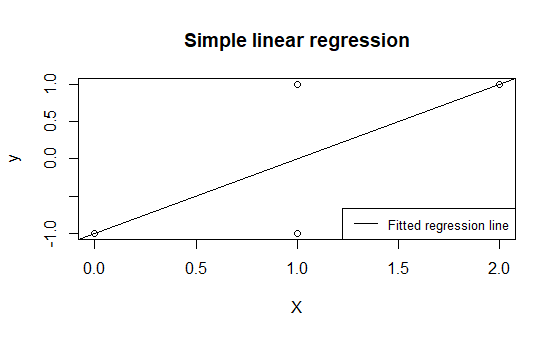
\includegraphics[scale=0.6]{p32b.png}
  %\caption{Simple linear regression}
\end{figure}
With {\fontfamily{ptm}\ttfamily lm} in R, in the plot we get the regression line with the intercept being -1 and the gradient being 1, which is the same as the result from manual computing.\\

\end{enumerate}

\newpage

\textbf{\textit{Appendix.}}\\

R codes for 1.a:
\lstinputlisting{p11a.R}
\vspace{3mm}

R codes for 1.b:
\lstinputlisting{p12a.R}
\vspace{3mm}

R codes for 1.c:
\lstinputlisting{p13a.R}
\vspace{3mm}

R codes for 1.d:
\lstinputlisting{p14a.R}
\vspace{3mm}

R codes for 2.a:
\lstinputlisting{p21a.R}
\vspace{3mm}

R codes for 2.b:
\lstinputlisting{p22a.R}
\vspace{3mm}

R codes for 2.c:
\lstinputlisting{p23a.R}
\vspace{3mm}

R codes for 3.b:
\lstinputlisting{p32a.R}
\vspace{3mm}

\end{document} 